\RequirePackage{ifpdf}
\documentclass[a4paper,11pt]{kth-mag}
\usepackage[T1]{fontenc}
\usepackage{textcomp}
\usepackage{lmodern}
\usepackage[utf8]{inputenc}
\usepackage[swedish,english]{babel}
\usepackage{modifications}
\usepackage{url}
\usepackage{graphicx}

\usepackage[dvipdfm,bookmarks]{hyperref}

% use sane colors for hyperlinks
\usepackage{xcolor}
\definecolor{dark-red}{rgb}{0.4,0.15,0.15}
\definecolor{dark-blue}{rgb}{0.15,0.15,0.4}
\definecolor{medium-blue}{rgb}{0,0,0.5}
\hypersetup{
    colorlinks, linkcolor={dark-red},
    citecolor={dark-blue}, urlcolor={medium-blue}
}

% enable blank pages by:
% \afterpage{\blankpage}
\usepackage{afterpage}

\newcommand\blankpage{%
    \null
    \thispagestyle{empty}%
    \addtocounter{page}{-1}%
    \newpage}

% Define a new pagestyle called 'center'
\makepagestyle{center}
\makeevenfoot{center}{}{\thepage}{}
\makeoddfoot{center}{}{\thepage}{}

\DeclareGraphicsExtensions{.eps}
%\DeclareGraphicsExtensions{.png}

\title{Configuration and device identification on network gateways}

\subtitle{Configuration and device identification on network gateways}
\foreigntitle{Konfigurering och enhetsidentifiering på nätverksgateways}
\author{Simon Kers}
\date{May 2013}
\blurb{Bachelor's Thesis at STH\\
       Supervisor: Micael Lundvall\\
       Examiner: Ibrahim Orhan
}
\trita{TRITA xxx 2013-nn}
\trita{}
\begin{document}

%\frontmatter
\pagenumbering{roman}
\setcounter{page}{3}
\pagestyle{center}

\maketitle
\selectlanguage{english}
\begin{abstract}
   Abstract in English.

\end{abstract}
\newpage
\blankpage

\begin{foreignabstract}{swedish}
   Innehåller en svensk sammanfattning av rapportens innehåll på 10-15 rader samt nyckelord som beskriver innehållet (upp till 10 stycken).
   Sammmanfattningen bör kortfattat redogöra för frågeställningen/problemmet, metoden och svaret/resultateet så precist som möjligt.

\newpage
\blankpage

\end{foreignabstract}
\clearpage
\tableofcontents*
\mainmatter
\pagestyle{newchap}
\chapter{Introduction}
%brief introduction to inteno and the product
Inteno Broadband Technology is a company that supplies customer premises equipment for internet service providers.  
Their headquarters and research and development center is located in Stockholm, Sweden.  
Inteno Open Systems Platform is a Linux-based open source platform running on customer premises equipment.
It is based on the OpenWrt distribution which targets embedded devices, specifically network gateways. \cite{Inteno}

%identified a real problem (motivate that it is real and interesting)
The technical support departments of partners and resellers of Intenos
customer premises equipment, are looking to reduce support costs and improve customer experience. 
Support issues creates costs for the business and by reducing the number of support tickets and their processing duration, these costs can be reduced.

%come up with a solution (give a rough idea what the solution looks like)
By simplifying configuration through abstracting common tasks for the end-user, the number of support calls can be reduced.
Using automatic device identification and automating common tasks such as port forwarding, support costs can be reduced and end-user satisfaction is higher.
Many common support issues could be automated by the software running on the customer premises equipment and by effectively communication with the end-user through the user interface.

%how I actually solved the problem (high-level summary of results).
The OpenWrt distribution provides a complete platform for compiling and deploying a gateway image.
By building a extensible library of presets for common port forwarding rules
and developing a simple selection dialog, the amount of calls can be lowered
while increasing customer satisfaction.

%skriv klart angående att tack vare ramverket så kan åf lägga till egna regler.


%\part{Important Results}

\chapter{Method}

\section{Preliminaries}

\subsection{OpenWrt}
OpenWrt is a free and open-source GNU/Linux distribution, targeting embedded devices, specifically wireless routers, but can run on almost any set of hardware.
Cross-compilation is enabled by OpenWrt Buildroot, which compiles the C code using uClibc, a lightweight C library focusing on embedded Linux systems. 
It intends to be a meta distribution and offers developers a framework on which to base their firmware on.

OpenWrt is generally compiled and linked using gcc and binutils, with the help of Makefiles and patches for the various gcc versions and target platforms.
Allowing end users as well as service operators and hardware manufacturers to compile the firmware.
It offers the BusyBox set of barebones UNIX tools, enabling advanced users to fully interact with their Linux system and providing developers with a familiar platform for debugging and testing their product.
\cite{OpenWrt:structure_design}

\subsection{OPKG}
The package management system used in OpenWrt is OPKG. It is based off the discontinued ipkg and operates similar to APT and dpkg of Debian-based distributions.
There are currently over 2000 OPKG packages available for OpenWrt.

The OpenWrt system and its packages are built using GNU Autoconf.

\subsection{Inteno Open Platform System}
For Customer Premises Equipment\footnote{commonly abbreviated as CPE} like wireless gateways, Inteno Open Platform System offers an open-source Linux distribution based on OpenWrt.
It uses the OpenWrt build system including cross-compilation toolchain to ensure compatibility with the ecosystem and upstream.

\subsection{Lua Configuration Interface}
LuCI is an suite of programs and libraries for extending OpenWrt using the Lua programming language.
It originated in the OpenWrt project but has since grown and is now it's own project.

The themes are accessed from the directory:

\begin{verbatim}
    root@Inteno:/usr/lib/lua/luci/view/themes/
\end{verbatim}

Rules for port forwarding are read from:

\begin{verbatim}
    /etc/config/firewall
\end{verbatim}

A port forwarding rule which forwards external HTTP traffic over port 80 to the local IP 192.168.1.214, looks like:

\begin{verbatim}
config redirect               
        option target 'DNAT' 
        option src 'wan'
        option dest 'lan'
        option proto 'tcp'
        option src_dport '80'
        option dest_ip '192.168.1.214'
        option dest_port '80' 
        option name 'Web server'
\end{verbatim}

The presentation markup for the current port forwarding page in the LuCI backend on the Gateway, is defined in the file:

\begin{verbatim}
    luci-inteno/applications/luci-firewall/luasrc/view/firewall/cbi_addforward.htm

    libs/core/luasrc/model/firewall.lua :555
\end{verbatim}

in the functions:

\begin{verbatim}
    function redirect.*
\end{verbatim}

\subsection{Remarks}

\subsection{Definitions}
See figure~\ref{fig:wizard-seq_dia} on page~\pageref{fig:wizard-seq_dia}.
\begin{figure}[h!]
   \centering
   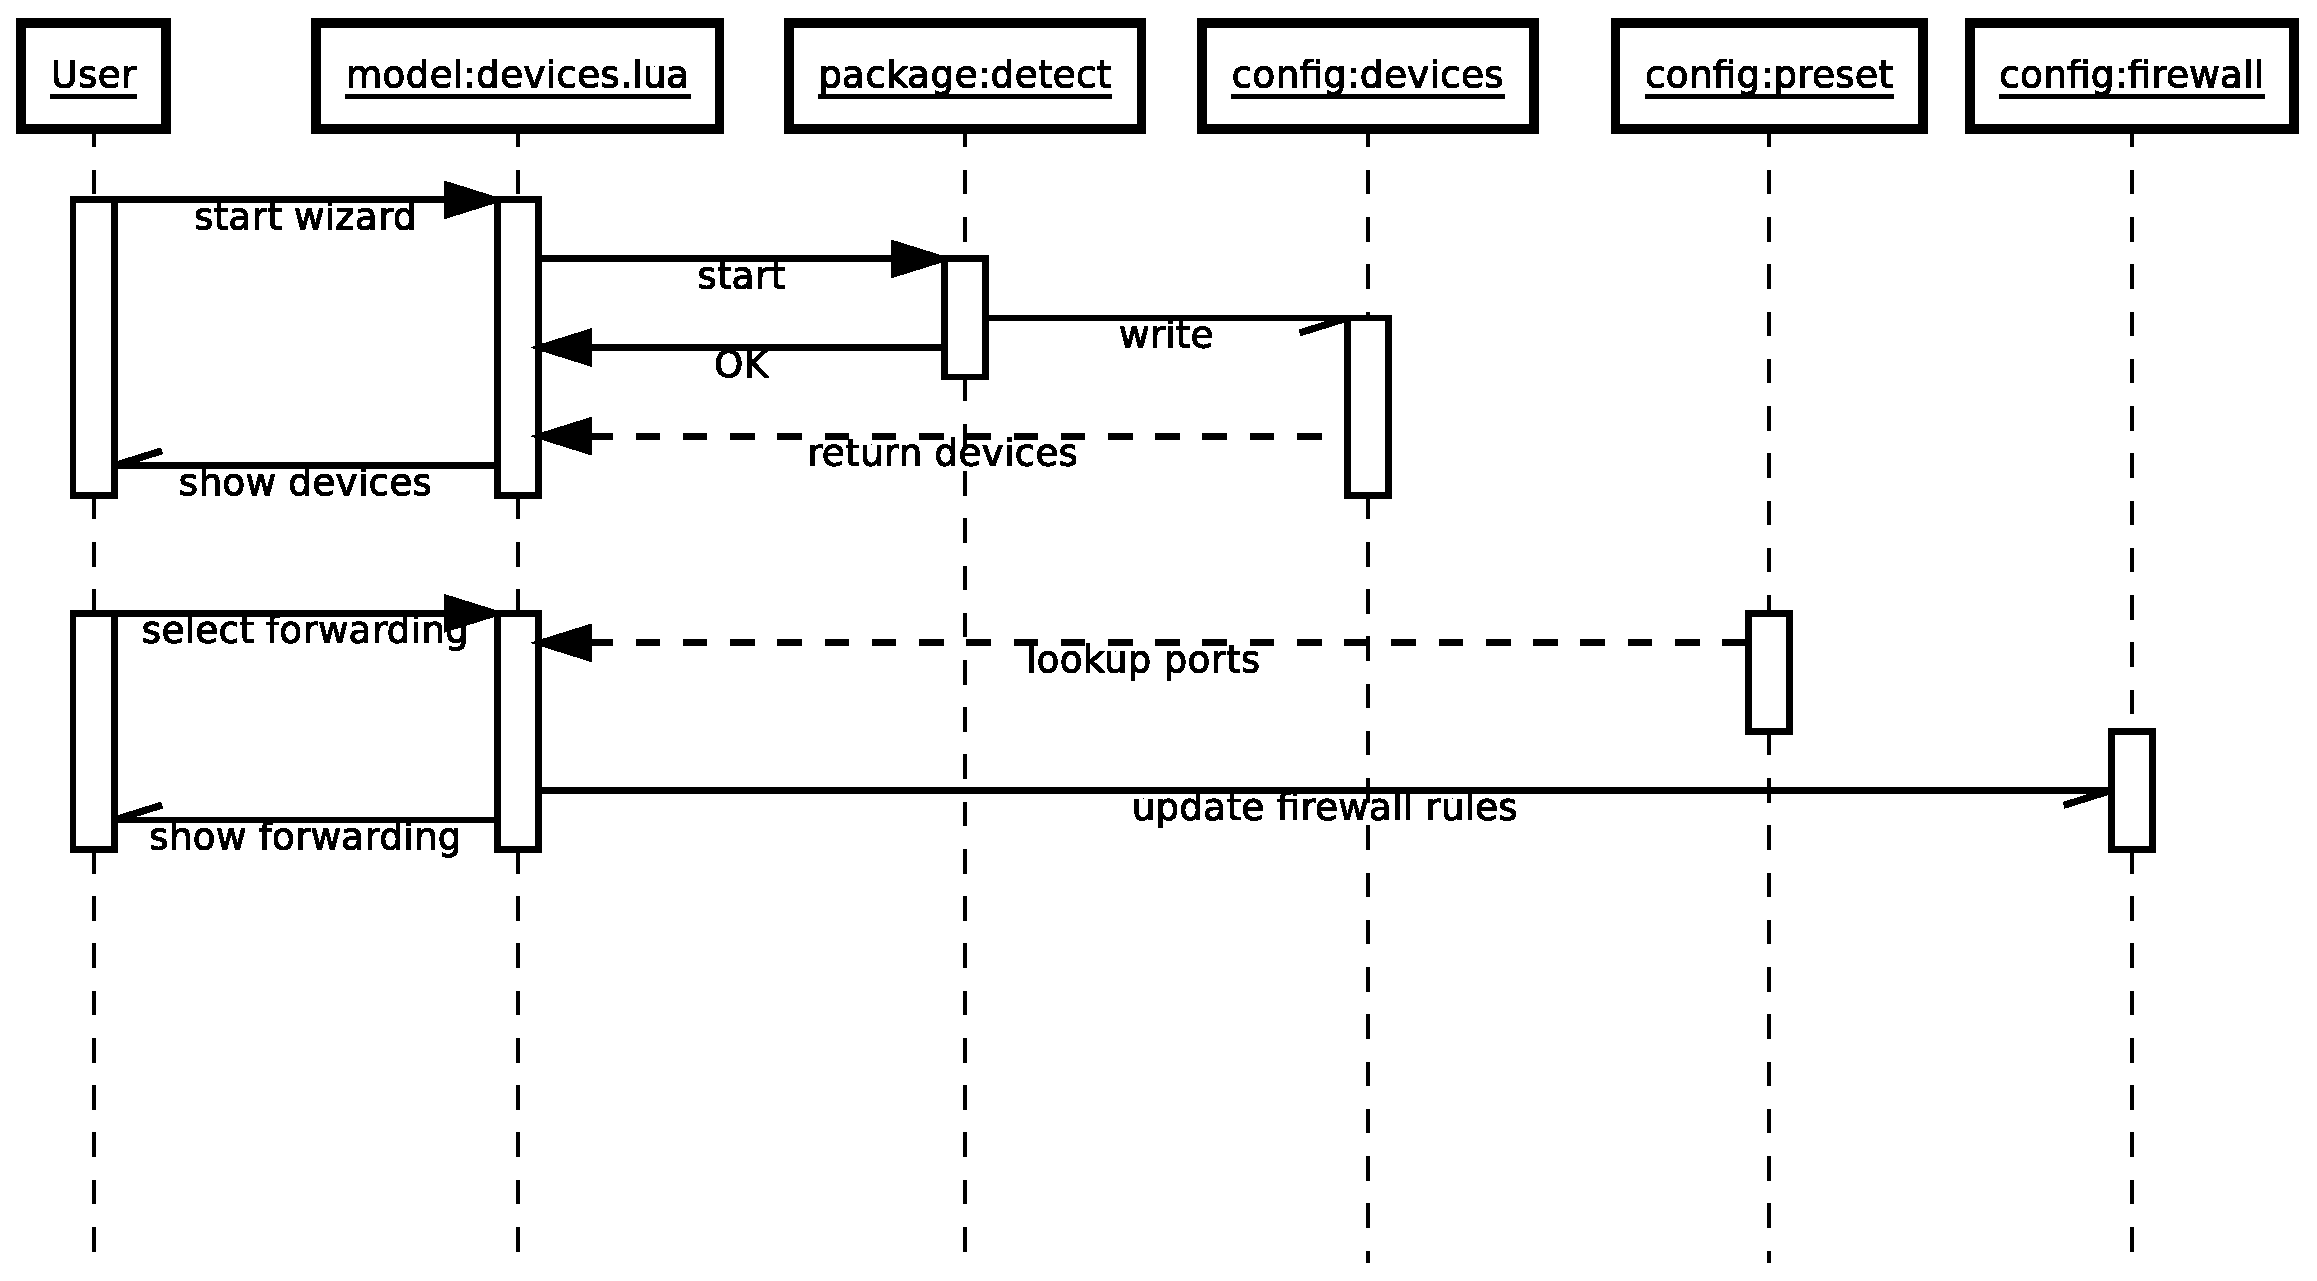
\includegraphics[width=15cm]{wizard-seq_dia}
   \caption{Sequential diagram of applying port forwarding rules}
   \label{fig:wizard-seq_dia}
\end{figure}

\section{The Main Theorem}

\subsection{Problem Statement}

\subsection{The Proof}
\subsubsection{Automatic port forwarding}


\appendix
\addappheadtotoc
\chapter{RDF}\label{appA}
\begin{figure}[ht]
   \begin{center}
And here is a figure
      \caption{
         \small{
            Several statements describing the same resource.
         }
      }
      \label{RDF_4}
   \end{center}
\end{figure}

that we refer to here: \ref{RDF_4}

\bibliographystyle{plain}
\bibliography{bibliography}
\end{document}
